\scanpage{115}
\mspage{705}

\[
\tag{267}
\left\{
\begin{gathered}
\unsure{\rho'}=\zeta\rho,\ \sigma'=\eta\sigma
\quad(\zeta,\eta\in\Gamma\underline M)\quad\text{tels qu'on ait}
\\
\rho'{}^3=\sigma'{}^2=\omega,\qquad
\sigma'(\rho')=\rho'{}^{-1}.
\end{gathered}\right.
\]

(On \unsure{note|notera} qu'un scindage doit transformer $\omega$,
qui opère trivialement sur $\underline M$ et est central
dans $\underline H^+$, dans une \deleted{\unsure{élément}}
\inserted{section} centrale, \unsure{or}
\deleted{\unsure{l'inverse}} \unsure{voir|voici} \unsure{pq} qu'on a
\[
\tag{268}
\left\{\begin{aligned}
\underline M\cap\underline{\mathrm{Cent}}\bigl(\underline{\mathfrak S}^+\bigr)
&=\underline M^{\mathfrak S_3}
=\deleted{\unsure{\{0\}}}\,\unsure{\{1\}|\{0\}},\quad\text{d'où}
\\
\underline{\mathrm{Cent}}\bigl(\underline{\mathfrak S}^+\bigr)
&\simeq\underline\mu_{\underline{\mathfrak S}}
=\{1,\omega\}_{\underline{\mathfrak S}}
\end{aligned}\right.
\]
--- ce qui montre qu'un scindage doit transformer $\omega$ en $\omega$,
d'où \unsure{facilement} la caractérisation (267) des $\rho',\sigma'$
\unsure{correspondants|correspondant} à un scindage).
On en aura
\[
\left\{\begin{aligned}
\rho'{}^3&=(\zeta\rho)^3
=\zeta\rho(\zeta)\rho^2(\zeta)\underbrace{\rho^3}_{\omega}
=\zeta\rho(\zeta)\rho^2(\zeta)\omega
\\
\sigma'{}^2&=(\eta\sigma)^2
=\eta\sigma(\eta)\underbrace{\sigma^2}_{\omega}
=\eta\sigma(\eta)\omega
\end{aligned}\right.
\]
donc les \deleted{deux} équations $\rho'{}^3=\omega$ et
$\sigma'{}^2=\omega$ équivalent respectivement à
\[
\left\{\begin{aligned}
\zeta\rho(\zeta)\rho^2(\zeta)&=1
&\text{i.e.}\quad(1+\rho_M+\rho_M^2)(\zeta)&=0
\\
\eta\sigma(\eta)&=1
&\text{i.e.}\quad(1+\sigma_M)(\eta)&=0
\end{aligned}\right.
\]
i.e. cela se réduit aux équations (245) (246),
et on a vu que la \deleted{solution générale est}
\inserted{\deleted{première} condition}
sur $\zeta$ est automatiquement satisfaite, celle
sur $\eta$ revient à :
\[
(247)\qquad
\eta=b\delta=b(\lambda_1-\lambda_0),\quad
\unsure{\lambda|b}\in\Gamma\mathbb G_a.
\]
La condition $\sigma'(\rho')=\rho'{}^{-1}$ s'explicite d'autre
part comme à la p.~$700'$, on retombe

\margin{114}

\begin{center}
\small
114\\
\texttt{https://grothendieck.umontpellier.fr}\\
Université de Montpellier, UMR CNRS 5149, Case courrier 051, Place Eugène Bataillon\\
34095 Montpellier cedex 5 - France
\end{center}

\scanpage{116}

sur l'équation (249), qui s'explicite par (250).
Cela montre qu'il existe un scindage
$\overline{\mathrm m}$ sur $S_0=\mathrm{Spec}\,\mathbb Z$
--- ce qui revient à un scindage \unsure{du} groupe discret
$\mathfrak S^+$ ext. de
$H^+=\mathfrak S^+/M$
\inserted{$\simeq\mathfrak S_0/\Pi_0$}
(par $M\simeq(\Pi_0)_{\mathrm{ab}}$ \unsure{)}
--- et que les scindages en question forment un
torseur sous $\underline K$, où $K$\inserted{$\simeq\mathbb Z^2$}
est défini dans (253), et en fait \deleted{\unsure{$K$}}
on a un isom $M\simeq K$ (254), soit
$\underline M\simeq\underline K$, \unsure{correspondant}
à l'opération de $\underline M$ sur le \unsure{schéma}
des scindages, par conjugaison. Ainsi on trouve

\uline{Proposition} (Sur une base $S$ quelconque).

L'extension $\underline{\mathfrak S}^+$ de
$\underline H^+$ par $\underline M$ est scindée ---
deux scindages sont conjugués par une unique section
de $\underline M$ --- donc l'application \deleted{de}
``passage au quotient par $\mu_{\mathfrak S}$'' définit une
bijection de l'\unsure{ens.} des scindages de
$\underline{\mathfrak S}^+$ sur $\underline H^+$,
sur l'\unsure{ens.} des scindages de
$\underline{\mathfrak S}^+/\mu_{\underline{\mathfrak S}}$
sur $\underline H^+/\underline\mu_{\underline H^+}
\simeq\underline{\mathfrak S}_3$.

\margin{115}

\begin{center}
\small
115\\
\texttt{https://grothendieck.umontpellier.fr}\\
Université de Montpellier, UMR CNRS 5149, Case courrier 051, Place Eugène Bataillon\\
34095 Montpellier cedex 5 - France
\end{center}

\scanpage{117}
\mspage{706}

Étudions maintenant le centralisateur dans
$\underline G_{\rho,\sigma}$ d'un sous-groupe section
au dessus de $\underline H^+$, \unsure{disons} noté
$\underline H(\rho',\sigma')$. On doit avoir maintenant
\[
\tag{269}
\underline{\mathrm{Cent}}_{\underline G_{\rho,\sigma}}
\bigl(\underline H(\rho',\sigma')\bigr)
\subset
\begin{gathered}
\mathbb O_{12}^*\cdot\bigl(\underline M\times
\underbrace{\mu_{\underline{\mathfrak S}}}_{=\{1,\omega\}_{S_0}}\bigr)
\\[-2pt]
\Vert
\\[-2pt]
\left\{\lambda\omega^i u_{\underline\mu}\ \middle|\
\begin{gathered}
\lambda\in\Gamma\underline M\\
\underline\mu\in\Gamma\mathbb O_{12}^*\\
i\in\Gamma(\unsure{\mathbb Z/2\mathbb Z})_{S_0}
\end{gathered}\right\}
\end{gathered}
\]
D'ailleurs $\lambda\omega^i u_{\underline\mu}$ centralise
$\underline H(\rho',\sigma')$ sss $\lambda u_{\underline\mu}$
centralise. La commutation à $\rho'$ s'explicite encore
par la condition (260), le calcul p.~703 s'appliquant
\unsure{ne varietur}. Pour la condition de commutation à
$\sigma'$, le calcul de p.~$703'$ doit se modifier
car on ne peut plus écrire $\omega^{\nu_2}=1$,
la condition s'écrit
\[
\omega^{\nu_2}\cdot\lambda\eta^{\unsure{\mu}}
\sigma(\lambda^{-1})\sigma=\eta\sigma
\quad\text{i.e.}\quad
\omega^{\nu_2}\lambda\eta^\mu\sigma(\lambda^{-1})=\eta
\]
et équivaut à la conjonction de la condition
\[
\tag{270}
\nu_2(\underline\mu)=0\quad\text{i.e.}\quad
\underline\mu\in\Gamma\mathbb O_{12}^{*\prime\prime},
\]
et de la relation (261). En présence de
$\nu_2(\underline\mu)=0$, les calculs des p.~$703'$, 704
s'appliquent, \unsure{finalement} on trouve :

\uline{Corollaire} Pour tout scindage de
$\underline{\mathfrak S}^+$ au dessus de
$\underline H^+$, \deleted{le commutant}
\inserted{\deleted{\illegible{1}} soit $\underline T$ le centralisateur
\deleted{\unsure{$T$}}} dans $\underline G_{\rho,\sigma}$
du sous-groupe section $\underline H(\rho',\sigma')$,
\deleted{on}

\margin{116}

\begin{center}
\small
116\\
\texttt{https://grothendieck.umontpellier.fr}\\
Université de Montpellier, UMR CNRS 5149, Case courrier 051, Place Eugène Bataillon\\
34095 Montpellier cedex 5 - France
\end{center}

\scanpage{118}

\deleted{\unsure{une section}}\inserted{On a alors} une suite exacte
\[
\tag{271}
\diagram{\begin{tikzcd}[column sep=large]
1 \arrow[r] & \underline\mu_{\unsure{\mathfrak S|G}}
\arrow[r,hook,"{\deleted{\unsure{G}}}" description]
& \underline T \arrow[r] & \mathbb O_{12}^{*\prime\prime}
\arrow[r,no head] & 1
\end{tikzcd}}
\]
et pour $\underline T^{\unsure{\natural|\sharp}}
=\underline T\cap\underline G_{\rho,\sigma}^{\unsure{\natural|\sharp}}$,
on a
\[
\tag{272}
\underline T^{\unsure{\natural|\sharp}}
\simeq\mathbb O_{12}^{*\prime\prime},
\]
i.e. $\underline T^{\unsure{\natural|\sharp}}$ est une section
partielle de $\underline G_{\rho,\sigma}^{\unsure{\natural|\sharp}}$
au dessus de $\mathbb O_{12}^{*\prime\prime}$.

\uline{Corollaire} L'extension $\underline G_{\rho,\sigma}$ de
$\mathbb O_{12}^*\times\underline H^+$ par $\underline M$
n'est scindée sur aucune base $S$ non vide.
L'extension $\underline G_{\rho,\sigma}''$ de
$\mathbb O_{12}^{*\prime\prime}\times\underline H^+$ par
$\underline M$ est scindée sur tte base $S$,
et deux scindages sont conjugués par une unique section de
$\underline M$. L'application naturelle fournit une bijection
de l'\unsure{ens.} des scindages de $\underline G_{\rho,\sigma}''$
sur $\mathbb O_{12}^{*\prime\prime}\times\underline H^+$, avec
l'\unsure{ens.} des scindages de
$\underline{\mathfrak S}^+$ sur $\underline H^+$.

\uline{Corollaire} L'ext. $G_{\rho,\sigma}$ de
$\widehat{\mathbb Z}^{*}\times H^+$ par $M^\wedge$
n'est pas scindée. Celle de $G_{\rho,\sigma}''$ de
$\widehat{\mathbb Z}^{*\prime\prime}\times H^+$ par
$M^\wedge$ est scindée, et deux scindages sont
conjugués par un unique élément \unsure{de} $\widehat M$.
L'application naturelle définit une bijection de l'\unsure{ens.}
des scindages de $G_{\rho,\sigma}''$ sur
$\widehat{\mathbb Z}^{*}\times H^+$ avec l'\unsure{ens.}
des scindages de \deleted{\unsure{$G_\rho$}}
$\mathfrak S^\wedge$ sur $H^+$.

\margin{117}

\begin{center}
\small
117\\
\texttt{https://grothendieck.umontpellier.fr}\\
Université de Montpellier, UMR CNRS 5149, Case courrier 051, Place Eugène Bataillon\\
34095 Montpellier cedex 5 - France
\end{center}

\scanpage{119}
\mspage{707}

Explicitons un scindage de l'extension
$\mathfrak S^+$ de $H^+$ par $M$
--- correspondant à un scindage de
$\underline{\mathfrak S}^+$ de $\underline H^+$
par $\underline M$ --- , via une solution particulière de l'équation
\[
\tag{273}
a_0-2a_1+3b-1=0
\]
en prenant
\[
a_1=b=0\qquad\text{d'où}\qquad a_0=1
\]
i.e.
\[
\tag{274}
\left\{\begin{aligned}
\zeta&=\lambda_0,\ \eta=0\quad\text{(écriture additive)}\\
\rho'&=\lambda_0\rho,\quad\unsure{\sigma'}=\unsure{\sigma}
\end{aligned}\right.
\]
\deleted{le scindage correspondant}
\inserted{les \unsure{trois} formules fournissent un scindage de
$\mathfrak S^+/\mu_{\mathfrak S}$}
au dessus de $\mathfrak S_3
\simeq H^+/\mu_{H^+}$.
Explicitons les \deleted{scindages}\inserted{relèvements}
\unsure{correspondants} de $\mathbb O_{12}^*$ dans
$\underline G_{\rho,\sigma}/\mu_G$ resp. de
$\mathbb O_{12}^{*\prime\prime}$ dans $\underline G_{\rho,\sigma}$\unsure{;},
\[
\tag{275}
\left\{\begin{aligned}
u_{\rho',\sigma'}:\mathbb O_{12}^*&\longrightarrow
\underline G_{\rho,\sigma}/\mu_G
\quad\text{resp.}\quad\mathbb O_{12}^{*\prime\prime}
\mathrel{\text{---}}\underline G_{\rho,\sigma}
\\
\underline\mu&\longmapsto\lambda_\infty^{\nu}u_{\underline\mu}
\qquad(\nu=\nu(\underline\mu))
\end{aligned}\right.
\]
où $u_{\underline\mu}$ défini dans (151).
(NB\unsure{\S} (275) est contenu dans prop. p.~704
(265) et (264), qui donnent
\[
u_{\rho',\sigma'}=\lambda u_{\underline\mu}\qquad
\lambda=x\lambda_0+y\lambda_1\qquad x=y=-\nu
\]
\[
\text{d'où}\qquad\lambda=-\nu(\lambda_0+\lambda_1)=\nu\lambda_\infty.
\]

On aura donc, posant
\[
u'_{\underline\mu}=u_{\rho',\sigma'}(\underline\mu)
\]
\[
\tag{276}
\left\{\begin{aligned}
u'_{\underline\mu}(\rho')&=\rho',\quad
u'_{\underline\mu}(\sigma')=\sigma'\\
u'_{\underline\mu}(\lambda)&=\mu\lambda\quad
(\lambda\in\Gamma\underline M)
\quad\inserted{\text{où}}\ (\mu=\unsure{\chi}(\underline\mu))
\end{aligned}\right\}
\quad\begin{gathered}
\text{(ce qui suffit}\\
\text{à \unsure{conditionner|caractériser}}\ u'_{\underline\mu})
\end{gathered}
\]

\margin{118}

\begin{center}
\small
118\\
\texttt{https://grothendieck.umontpellier.fr}\\
Université de Montpellier, UMR CNRS 5149, Case courrier 051, Place Eugène Bataillon\\
34095 Montpellier cedex 5 - France
\end{center}

\scanpage{120}

et on en déduit aussi
\[
\tag{277}
\left\{
\begin{aligned}
u'_{\underline{\mu}}(\rho)&=\lambda_0^{-2\nu}\rho\\
u'_{\unsure{\mu|\underline{\mu}}}(\sigma)&=\omega^{\nu_2}\sigma
\qquad (=\sigma\text{ dans }\underline G_{\rho,\sigma}/\underline{\mu}_G\ \ldots).
\end{aligned}
\right.
\]

\margin{119}

\begin{center}
\small
119\\
\texttt{https://grothendieck.umontpellier.fr}\\
Université de Montpellier, UMR CNRS 5149, Case courrier 051, Place Eugène Bataillon\\
34095 Montpellier cedex 5 - France
\end{center}

\scanpage{121}
\mspage{708}

13\textsuperscript{o}) \uline{Retour sur la tour de Fermat}.

Commençons par dégager une notion topossique générale, qui \unsure{était} un peu
embrouillée entre les lignes dans 11\textsuperscript{o}).
Soit $\Gamma$ (ici $\Gamma_{\mathbb Q}\times
\mathfrak S_3\deleted{\unsure{)|\}}}=N_{0,3}$) opérant sur
un topos $\mathcal X$ (ici
$\deleted{\unsure{U}}\inserted{\unsure{\mathcal U}_{0,3\overline{\mathbb Q}}}
\simeq M'_{0,4\overline{\mathbb Q}}$) conn.
\inserted{loc. connexe}, \deleted{\unsure{et conn.}} muni d'un ``pt'' (géométrique)
$x_0$ (ici: le point $-\overline j$ à valeurs dans $\overline{\mathbb Q}$), soient
\margin{Contexte discret ($\mathcal X$ loc. simpl. connexe) ou profini,
\unsure{rel.}\illegible{1} \unsure{raisonnables}\ldots}
\[
\tag{278}
\left\{
\begin{aligned}
\Pi&=\Pi_1(\mathcal X,x_0),\qquad
\mathcal M=\Pi_1(\mathcal X,\Gamma;x_0)\\
M&=\Pi_{\mathrm{ab}}=\Pi/[\Pi,\Pi],\qquad
\deleted{\unsure{\mathfrak S}}\inserted{\widetilde{\mathcal M}}
=\mathcal M/[\Pi,\Pi],\qquad \deleted{\text{d'où}}
\end{aligned}
\right.
\]
d'où des suites exactes et hom. de suites exactes
\[
\tag{279}
\diagram{\begin{tikzcd}[column sep=large,row sep=large]
1 \arrow[r,dash] & \Pi \arrow[r] \arrow[d,"\text{épi}"]
& \mathcal M \arrow[r] \arrow[d,"\text{épi}"]
& \Gamma \arrow[r,dash] \arrow[d,"\unsure{\sim|\wr}"] & 1\\
1 \arrow[r,dash] & M \arrow[r,dash]
& \deleted{\unsure{\mathfrak S}}\inserted{\widetilde{\mathcal M}} \arrow[r]
& \Gamma \arrow[r,dash] & 1
\end{tikzcd}}\ .
\]

\deleted{Considérons}
\inserted{(Au lieu de prendre
$M=\Pi/\unsure{(\Pi,\Pi)|[\Pi,\Pi]}\inserted{=\Pi_{\mathrm{ab}}}$,}
on \unsure{aurait|avait} pu prendre un quotient de $\Pi_{\mathrm{ab}}$ invariant par
action de $\Gamma$, mais peu importe\ldots).
Considérons ``le rev. universel abélien'' \inserted{$\mathcal X'_0$} de
$\mathcal X$ en $x_0$, i.e. le quotient par $[\Pi,\Pi]$ du rev. universel de
$\mathcal X$ en $x_0$ --- c'est donc un rev. principal de $\mathcal X$, de
groupe $M$. On

\margin{120}

\begin{center}
\small
120\\
\texttt{https://grothendieck.umontpellier.fr}\\
Université de Montpellier, UMR CNRS 5149, Case courrier 051, Place Eugène Bataillon\\
34095 Montpellier cedex 5 - France
\end{center}

\scanpage{122}

se propose d'examiner les façons de \deleted{prolonger}\inserted{relever}
l'action de $\Gamma$ sur $\mathcal X$ \deleted{(via $M$)} en une
action \deleted{de $\mathcal M$}\inserted{sur $\mathcal X'_0$}, compatible
avec l'action \inserted{de $\Gamma$ sur le groupe d'opérateurs $M$}
\deleted{sur $\mathcal X$ via $\Gamma$,
\inserted{et prolonger l'action de
$M\subset\mathfrak S$,}
\unsure{ou ce qui} \unsure{revient} au $\overline{\mathrm m}$, par une action de
$\mathfrak S$, compatible avec son action sur
$\mathcal X$ (via $\Gamma$)}.
Plus généralement, si $\mathcal X'$ est un $M_{\mathcal X}$-torseur sur
$\mathcal X$ isomorphe \unsure{à} $\mathcal X'_0$, donc déduit
\deleted{\unsure{par un}}\inserted{de $\mathcal X'_0$} par twist à l'aide
d'un $M$-torseur $E$ ($\unsure{\simeq|=}$ fibre de $\mathcal X'_0$ en $x_0$),
étudions les \deleted{extensions}\inserted{relèvements} analogues de l'action
de $\deleted{\unsure{\mathfrak S}}\inserted{\Gamma}$ sur $\mathcal X$ en une
action de $\deleted{\unsure{\mathfrak S}}\inserted{\Gamma\text{ sur }\mathcal X'}$,
compatible avec l'action de
$\deleted{\unsure{\mathfrak S}}\inserted{\Gamma}$ sur $\mathcal X$.

\deleted{Notons que, si $\widetilde{\mathcal X}$ désigne le rev. universel de
$\mathcal X$ en $x_0$, $\mathcal M$ opère sur $\widetilde{\mathcal X}$ de façon
compatible avec son action sur $\mathcal X$, \unsure{en|et} prolongeant l'action
\inserted{canonique} de $\Pi$ sur $\widetilde{\mathcal X}$ --- comme
$[\Pi,\Pi]\subset\Pi$ est distingué dans $\mathcal M$, cette action passe au
quotient en une action canonique de
$\mathfrak S=\mathcal M/[\Pi,\Pi]$ sur
$\mathcal X'_0=\widetilde{\mathcal X}/[\Pi,\Pi]$, qui satisfait aux}

\margin{121}

\begin{center}
\small
121\\
\texttt{https://grothendieck.umontpellier.fr}\\
Université de Montpellier, UMR CNRS 5149, Case courrier 051, Place Eugène Bataillon\\
34095 Montpellier cedex 5 - France
\end{center}

\scanpage{123}
\mspage{709}

\deleted{\inserted{deux} conditions envisagées. Soit $\Theta_0$ cette
opération-ci de $\mathfrak S$, et $\Theta$ une opération
quelconque, satisfaisant aux dites conditions.}

On veut donc faire de $\mathcal X'$, qui est un rev. de $\mathcal X$, donné
par sa fibre $E$ en $x_0$ et l'action de $\Pi=\Pi_1(\mathcal X,x_0)$ sur
$E$ (par translations, grâce à une structure de $M$ torseur sur $E$) un
revêtement de $(\mathcal X',\deleted{\unsure{\mathfrak S}}\inserted{\Gamma})$
--- i.e. \uline{prolonger} l'action donnée de $\Pi$ sur \unsure{la|le} fibre
$E$, en une action de $\mathcal M$ sur $E$ --- qui d'ailleurs se factorise
nécessairement par
$\deleted{\unsure{\mathfrak S}}\inserted{\widetilde{\mathcal M}}$.
Je dis que cette action se fait néc\textsuperscript{t} \unsure{à} travers le
groupe affine du torseur $E$ --- de façon précise, $\Gamma$ opère sur $M$,
\unsure{soit} $\gamma_M$ l'opération définie par $\gamma\in\Gamma$, et soit
$g\in\deleted{\unsure{\mathfrak S}}\inserted{\widetilde{\mathcal M}}$ au dessus de
$\gamma\in\Gamma$, on aura donc, pour $x\in E$, $\lambda\in M$
\[
\tag{280}
\diagram{\begin{tikzcd}[column sep=0em,row sep=0.6em]
g & (\lambda & {}\cdot{} & x & {})=\gamma_M(\lambda)\mathbin{.}gx\\
\deleted{\unsure{\mathfrak S}}\inserted{\widetilde{\mathcal M}}
\arrow[u,phantom,"\in"{description,rotate=-90}]
& M\arrow[u,phantom,"\in"{description,rotate=-90}]
& & E\arrow[u,phantom,"\in"{description,rotate=-90}] &
\end{tikzcd}}
\]
ce qui \unsure{est} trivial par le calcul.
\deleted{\unsure{car|est}}
\[
g(\lambda.x)=(g\lambda)x=(g\lambda g^{-1}g)x
=\underbrace{(g\lambda g^{-1})}_{\gamma_M(\lambda)}.(gx)
\]

\margin{122}

\begin{center}
\small
122\\
\texttt{https://grothendieck.umontpellier.fr}\\
Université de Montpellier, UMR CNRS 5149, Case courrier 051, Place Eugène Bataillon\\
34095 Montpellier cedex 5 - France
\end{center}

\scanpage{124}

Donc si on introduit le groupe $\operatorname{Aff}(E)$, on aura un
homomorphisme de suites exactes
\[
\tag{281}
\diagram{\begin{tikzcd}[column sep=large,row sep=large]
1 \arrow[r] & M \arrow[r,dash]
\arrow[d,Rightarrow,"{\deleted{\unsure{\Theta}}\mathrm{id}_M}"]
& \deleted{\unsure{\mathfrak S}}
\inserted{\widetilde{\mathcal M}} \arrow[r]
\arrow[d,"{\Theta_{\deleted{\unsure{\mathfrak S}}\inserted{\widetilde{\mathcal M}}}}"]
& \Gamma \arrow[r,dash] \arrow[d,"\Theta_\Gamma"] & 1\\
1 \arrow[r,dash] & M \arrow[r]
& \operatorname{Aff}(E) \arrow[r]
& \operatorname{Aut}(M) \arrow[r] & 1
\end{tikzcd}}
\]
où les flèches verticales extrêmes $\mathrm{id}_M$ \inserted{et
$\Theta_\Gamma$} sont connues, et où la flèche médiane est à déterminer.
On peut dire que la catégorie des $\mathcal X'$ \unsure{cherchés|cherchées}
(avec l'op. de $\Gamma$ dessus satisfaisant aux conditions voulues)
\inserted{est} équivalente à celle des couples
$(E,\Theta_{\deleted{\unsure{\mathfrak S}}\inserted{\widetilde{\mathcal M}}})$,
où $E$ est un $M$-torseur, et
$\Theta_{\deleted{\unsure{\mathfrak S}}\inserted{\widetilde{\mathcal M}}}$
un hom de groupes
$\deleted{\unsure{\mathfrak S}}\inserted{\widetilde{\mathcal M}}
\longrightarrow\operatorname{Aff}(E)$ \deleted{\unsure{rendant}}
compatible avec $\mathrm{id}_M$ et $\Theta_\Gamma$ i.e. qui
\unsure{rende|rend} commutatif (281).
On peut dire aussi: une fois $E$ choisi,
\inserted{(et ce choix est \unsure{anodin} à isom non unique
près\unsure{!!!|\ldots})}
que cela définit une extension $\operatorname{Aff}(E)$ de
$\operatorname{Aut}(M)$ par $M$, d'où grâce à
$\Gamma\longrightarrow\operatorname{Aut}(M)$ une
extension

\margin{123}

\begin{center}
\small
123\\
\texttt{https://grothendieck.umontpellier.fr}\\
Université de Montpellier, UMR CNRS 5149, Case courrier 051, Place Eugène Bataillon\\
34095 Montpellier cedex 5 - France
\end{center}

\scanpage{125}
\mspage{\textcircled{710}}

\margin{les scindages de $\operatorname{Aff}(E)$ déterminés par les pts de $E$ -- \unsure{dépt} de l'origine \unsure{scindages} \unsure{intérieurs}\ldots}

par $M$, \inserted{qui est \uline{d'ailleurs scindée}.} (Ceci dit, les relèvements d'action de $\Gamma$ dessus correspondent aux isomorphismes de cette extension de $\Gamma$ par $M$, avec l'extension $\mathfrak S$ elle-$\overline{\mathrm m}$. Donc elle existe sss l'extension de $\mathfrak S$ de $\Gamma$ par $M$ est scindée, \deleted{\unsure{ce qui}} \inserted{i.e.\ \unsure{l'expression}}
\[
c^2(\mathfrak S)\in H^2(\Gamma,M)\quad\text{est nulle.}
\tag{282}
\]
S'il existe un tel relèvement i.e. un tel isomorphisme, ceux-ci forment un torseur \unsure{sous|sur} le groupe des autom. de l'extension (triviale) $\mathfrak S$ de $\Gamma$ par $M$ qui s'identifie au groupe
\[
(\qquad Z^1(\Gamma,M)
\]
des homomorphismes croisés de $\Gamma$ dans $M$. Les classes de $M$-conjugaison de tels \deleted{relèvements \unsure{(ou}} isomorphismes correspondent donc aux éléments de
\[
H^1(\Gamma,M).
\]

Une autre façon de le dire, en prenant $E={}$\inserted{$M$-}torseur trivial${}=M$, donc $\operatorname{Aff}(E)$ scindé, c'est que les relèvements choisis correspondent aux \uline{scindages} de l'extension $\mathfrak S$ de $\Gamma$ par $M$, et les classes de \inserted{$M$-}conjugaison des relèvements d'action de $\Gamma$ sur $\mathcal X'_0$

\margin{124}

\begin{center}
\small
124\\
\texttt{https://grothendieck.umontpellier.fr}\\
Université de Montpellier, UMR CNRS 5149, Case courrier 051, Place Eugène Bataillon\\
34095 Montpellier cedex 5 - France
\end{center}

\scanpage{126}

correspondent aux classes de $M$-conjugaison des scindages de ladite extension $\mathfrak S$ de $\Gamma$ par $M$.

Ceci bien posé, revenons à la situation de
\[
\left(\underbrace{U_{0,3\overline{\mathbb Q}}}_{\mathcal X},\quad
\Gamma=\underbrace{\Gamma_{\mathbb Q}\times\mathfrak S_3}_{N_{0,3}}\right),
\]
les $\Gamma$-revêtements de $\mathcal X$ correspondent aux $\mathfrak S_3$-revêtements de $U_{0,3\mathbb Q}$, i.e. aux rev. de $(U_{0,3\mathbb Q},\mathfrak S_3)$.

\margin{\uline{NB} Le groupe qu'on vient de noter $M$ devient ici $\unsure{\widehat M}$, $\mathcal M$ devient $\mathcal M_{0,3}$, $\pi$ devient $\widehat\Pi_{0,3}$.}

À l'aide des constructions générales du \S~49 $\overline{\uline{\mathrm{VI}}}$, \deleted{on a déduit} du quotient
\[
\deleted{\unsure{G_{\rho,\sigma}}=\unsure{\mathfrak S}^{+\wedge}/\unsure{\mu_G}\simeq
\operatorname{SL}(2,\mathbb Z)^\wedge/
[\unsure{\widehat\Pi_{0,3}},\unsure{\widehat\Pi_{0,3}}]}
\]
\[
\mathfrak S^{+\wedge}/\mu_{\mathfrak S}\simeq
\unsure{\mathcal M}_{0,3}^{+}/[\widehat\Pi_{0,3},\widehat\Pi_{0,3}]
\subset\widetilde{\mathcal M}
\]
\deleted{est}

\margin{on pourrait le noter $\unsure{\widetilde{\mathcal M}'}$!}

\deleted{ext} (avec les notations des pages précédentes), extension de $\mathfrak S_3\subset\Gamma(=\Gamma_{\mathbb Q}\times\mathfrak S_3)$ par $M^\wedge$, on a \inserted{déduit} un groupe profini, \deleted{\unsure{et}} qui était noté $G_{\rho,\sigma}/\mu_G$ \inserted{ou $G_{\rho,\widetilde\sigma}$} dans les sections précédentes et y apparaissait comme un produit $\frac12$-direct
\[
G_{\rho,\widetilde\sigma}
=\deleted{\unsure{\mathbb O|\Phi}}\widehat{\mathbb Z}^{*}\mathbin{.}\widetilde{\mathcal M},
\qquad\text{ext. de }\widehat{\mathbb Z}^{*}\times\mathfrak S_3
\quad\text{par }M^\wedge
\]
et un hom. canonique
\[
\widetilde{\mathcal M}
=\mathcal M_{0,3}/(\widehat\Pi_{0,3},\widehat\Pi_{0,3})
\longrightarrow G_{\rho,\widetilde\sigma}
\]
s'insérant dans un hom. de suites exactes

\margin{125}

\begin{center}
\small
125\\
\texttt{https://grothendieck.umontpellier.fr}\\
Université de Montpellier, UMR CNRS 5149, Case courrier 051, Place Eugène Bataillon\\
34095 Montpellier cedex 5 - France
\end{center}

\scanpage{127}
\mspage{711}

\diagram{
\[
\begin{tikzcd}[column sep=large,row sep=huge]
1 \arrow[r,no head] &
\widehat M \arrow[r] \arrow[d,Rightarrow] &
\widetilde{\mathcal M} \arrow[r] \arrow[d] &
\underbrace{\Gamma}_{N_{0,3}=\Gamma_{\mathbb Q}\times\mathfrak S_3}
\arrow[r,no head] \arrow[d,"\unsure{\chi}\times\operatorname{id}_{\mathfrak S_3}"] & 1 \\
1 \arrow[r,no head] &
\widehat M \arrow[r,no head] &
G_{\rho,\widetilde\sigma} \arrow[r] &
\widehat{\mathbb Z}^{*}\times\mathfrak S_3 \arrow[r,no head] & 1 .
\end{tikzcd}
\tag{282}
\]
}

D'ailleurs contre \unsure{tte|toute} attente on a trouvé que l'extension $G_{\rho,\widetilde\sigma}$ de $\widehat{\mathbb Z}^{*}\times\mathfrak S_3$ par $\widehat M$ était scindée, d'où il résulte que \deleted{celle de} l'ext. $\widetilde{\mathcal M}$. de $\Gamma$ par $\widehat M$ l'est aussi (\deleted{ce qui \unsure{précède|précédait}} \inserted{ce dernier fait} est aussi conséquence de l'existence de la tour de Fermat, en y appliquant les réflexions générales des pages précédentes). Bien mieux, on a vu qu'il y a une unique classe de $\widehat M$-conj. de scindages de l'extension $G_{\rho,\widetilde\sigma}$, ce qui induit une classe de $\widehat M$-conjugaison \uline{canonique} (mais non unique!) de \deleted{$\unsure{\widehat M}$} scindages de $\widetilde{\mathcal M}$ au-dessus de $\Gamma$. Cela définit donc une classe d'\deleted{isomorphie}\inserted{$\widehat M$-conjugaison} canonique de relèvements de l'action de $\Gamma$ \inserted{sur $\mathcal X=U_{0,3\overline{\mathbb Q}}$} à $\mathcal X'_0$ -- ou ce qui revient au $\overline{\mathrm m}$, un torseur sur $(U_{0,3\mathbb Q},\mathfrak S_3)$, de groupe un groupe profini

\margin{\uline{NB} $H^1(\Gamma,\widehat M)$ est un groupe fort gros! -- Mais voir \unsure{ci-dessous}, cf Th. p.~716}

\margin{126}

\begin{center}
\small
126\\
\texttt{https://grothendieck.umontpellier.fr}\\
Université de Montpellier, UMR CNRS 5149, Case courrier 051, Place Eugène Bataillon\\
34095 Montpellier cedex 5 - France
\end{center}

\scanpage{128}

commutatif au dessus de $(U_{0,3\mathbb Q},\mathfrak S_3)$ qui au dessus de \deleted{$U_{0,3\unsure{\overline{\mathbb Q}}}$ \illegible{2}} \inserted{$U_{0,3\overline{\mathbb Q}}$ soit isomorphe} au rev. $\mathcal X'_0$ envisagé plus haut.

Revenons pour un instant à ce cas général du début. Notons que la donnée d'un diagramme (281) \deleted{imposant} définit un quotient \inserted{$\widetilde{\widetilde{\mathcal M}}$} de $\widetilde{\mathcal M}$ -- à savoir le coimage de $\Theta_{\widetilde{\mathcal M}}$ -- \deleted{\unsure{donnant} lieu à une suite} \inserted{tel que $M\hookrightarrow\widetilde{\widetilde{\mathcal M}}$ soit injectif, et} donnant donc lieu à une suite \deleted{exacte} exacte
\diagram{
\[
\begin{tikzcd}[column sep=large,row sep=large]
1 \arrow[r,no head] & M \arrow[r,no head] &
\widetilde{\widetilde{\mathcal M}} \arrow[r,no head] &
\widetilde\Gamma \arrow[r,no head] \arrow[d,equal,"\mathrm{déf}"] & 1, \\
& & & \widetilde{\widetilde{\mathcal M}}/\operatorname{Im}M &
\end{tikzcd}
\tag{283}
\]
}
\unsure{puis|où} on a
\diagram{
\[
\begin{tikzcd}[column sep=large]
\widetilde\Gamma \arrow[r,hook] & \operatorname{Aut}(M),
\end{tikzcd}
\tag{284}
\]
}
$\widetilde\Gamma$ s'identifie à l'image de $\Gamma$ dans $\operatorname{Aut}(M)$ par l'action de $\Gamma$ sur $M$ provenant de la structure d'ext. $\widetilde{\mathcal M}$ de $\Gamma$ par $M$.

\deleted{Cette} Ce quotient $\widetilde{\widetilde{\mathcal M}}$ de $\mathcal M$, donnant naissance à une ext. (283), n'est pas quelconque -- à part le fait que $M$ s'y envoie injectivement, et que $\widetilde\Gamma=\widetilde{\widetilde{\mathcal M}}/\operatorname{Im}M$

\margin{127}

\begin{center}
\small
127\\
\texttt{https://grothendieck.umontpellier.fr}\\
Université de Montpellier, UMR CNRS 5149, Case courrier 051, Place Eugène Bataillon\\
34095 Montpellier cedex 5 - France
\end{center}

\scanpage{129}
\mspage{712}

opère \deleted{\unsure{injective|injectivement}} \inserted{\uline{fidèlement}} sur $M$ : en plus, l'extension (283) est triviale, et \deleted{en fait} \inserted{le fait} qu'elle provienne d'un $\Theta_{\widetilde{\mathcal M}}$ implique une \uline{structure supplémentaire} sur cette extension, à savoir la donnée d'une classe de $M$-conjugaison de scindages.

Plus précisément, on aura une application canonique
\diagram{
\[
\begin{tikzcd}[column sep=large]
E \arrow[r] & \operatorname{Scind}\bigl(\widetilde{\widetilde{\mathcal M}}\ \text{\unsure{comme|conçue} ext de }\widetilde\Gamma\text{ par }M\bigr)
\end{tikzcd}
\tag{285}
\]
}
compatible avec les opérations de $M$ sur $E$ (par translation) et sur $\operatorname{Scind}$ (par composition \unsure{avec|ou} \unsure{autom.|automs} intérieurs).
\inserted{La classe de $M$-conjugaison envisagée de scindages n'est autre que l'image de $E$.}

Pour que $x$ et $y\in E$ aient $\overline{\mathrm m}$ image dans $\operatorname{Scind}$, il f et s. que l'élément $u=y-x\in M$ soit dans $M^\Gamma=M^{\widetilde\Gamma}$, ce qui montre que
\diagram{
\[
\begin{tikzcd}[column sep=large,row sep=large]
\text{l'hom }E \arrow[r,no head] & \operatorname{Scind}\text{ est injectif} \\
& \text{sss}\quad M^\Gamma=\{0\}\quad .
\end{tikzcd}
\tag{286}
\]
}

Dans le cas où $M^\Gamma=\{0\}$, on voit donc que $E$ s'identifie exactement à une classe de $M$-conjugaison des scindages de $\widetilde{\widetilde{\mathcal M}}$.

\margin{128}

\begin{center}
\small
128\\
\texttt{https://grothendieck.umontpellier.fr}\\
Université de Montpellier, UMR CNRS 5149, Case courrier 051, Place Eugène Bataillon\\
34095 Montpellier cedex 5 - France
\end{center}

\scanpage{130}

Résumons ces considérations, dans une

\uline{Proposition} Soient $\mathcal X$ un topos \deleted{\unsure{c}} connexe loc. connexe muni d'un pt géom. $x_0$, on se place dans le contexte discret ($\mathcal X$ \unsure{loc.|loc} \unsure{simpl|simpl.} connexe) ou profini (revêtement signifie revêtement profini).
\margin{\figure{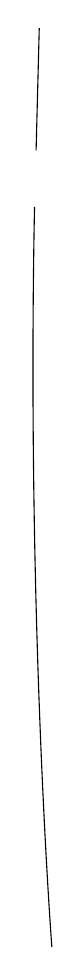
\begin{tikzpicture}[x=1cm,y=1cm]
\draw (0,0) -- (-0.04,-1.55);
\draw (-0.06,-2.27) .. controls (-0.14,-6.3) and (0.04,-10.0) .. (0.16,-11.67);
\end{tikzpicture}}}

On a un groupe $\Gamma$ d'\unsure{autom} de $\mathcal X$ ($\Gamma$ profini dans le cas profini --- il faudrait expliciter pour bien faire les hypothèses raisonnables à faire pour tenir compte de la topologie profinie de $\Gamma$\ldots). On pose
\[
\Pi=\Pi_1(\mathcal X,x_0),\quad \mathcal M=\Pi_1(\mathcal X,\Gamma;x_0)\qquad\text{d'où}
\]
\inserted{\diagram{\begin{tikzcd}[column sep=large]
{(*)}\quad 1 \arrow[r,no head] & \Pi \arrow[r,no head] & \mathcal M \arrow[r,no head] & \Gamma \arrow[r] & 1
\end{tikzcd}}}
on se donne un quotient $M$ de $\Pi$, \deleted{\unsure{un}} par un sous-groupe distingué \uline{dans $\mathcal M$}, \unsure{ou} ce qui revient au $\overline{\mathrm m}$ un quotient de $\Pi_{\mathrm{ab}}=\Pi/[\Pi,\Pi]$ stable par l'action de $\Gamma$, \deleted{pour}\inserted{d'où} une \deleted{$\widetilde{\mathcal M}=\mathcal M/$} extension quotient de $(*)$,
\[
(287)\qquad
\diagram{\begin{tikzcd}[column sep=large]
1 \arrow[r] & M \arrow[r,no head] & \widetilde{\mathcal M} \arrow[r,no head] & \Gamma \arrow[r,no head] & 1
\end{tikzcd}}
\]
où $M$ est \unsure{comm|comm.} donc $\Gamma$ opère sur $M$.

On s'intéresse à la catégorie des revêtements \deleted{$\unsure{M_{\mathcal X}}$-torseurs $\mathcal X'_0$ \unsure{sur}} $\mathcal X'$ de $(\mathcal X,\Gamma)$, satisfaisant les conditions

\margin{129}

\begin{center}
\small
129\\
\texttt{https://grothendieck.umontpellier.fr}\\
Université de Montpellier, UMR CNRS 5149, Case courrier 051, Place Eugène Bataillon\\
34095 Montpellier cedex 5 - France
\end{center}

\scanpage{131}
\mspage{713}

Suivantes : après oubli des opérations de $\Gamma$, on trouve un revêtement \inserted{connexe} galoisien \inserted{\unsure{(et $\overline{\mathrm m}$ abélien)}} de $\mathcal X$, correspondant au groupe quotient $M$ de $\Pi=\Pi_1(\mathcal X,x_0)$ --- de sorte que $\mathcal X'$ devient de façon naturelle un torseur sous $M_{\mathcal X}$.
\margin{\figure{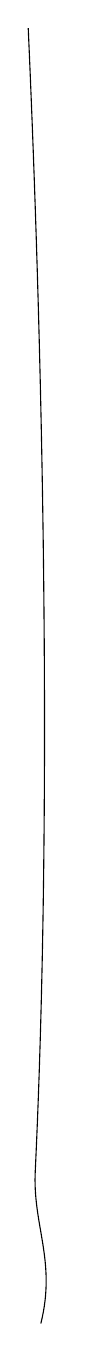
\begin{tikzpicture}[x=1cm,y=1cm]
\draw (0,0) .. controls (0.2,-4.5) and (0.3,-10.0) .. (0.09,-14.5) .. controls (0.05,-15.2) and (0.36,-15.65) .. (0.16,-16.45);
\end{tikzpicture}}}
Le foncteur
\[
\mathcal X'\longmapsto\mathcal X'(x_0)\qquad\text{(fibre en $x_0$)}
\]
de la catégorie de ces $\mathcal X'$ dans la catégorie des ensembles, s'en va en fait vers les ensembles $E$ munis des structures suivantes

\noindent a) $E$ est un $M$-torseur, et en tant que tel donne naissance à une extension
\diagram{\begin{tikzcd}[column sep=large]
1 \arrow[r,no head] & M \arrow[r] & \operatorname{Aff}(E) \arrow[r] & \operatorname{Aut}(M) \arrow[r,no head] & 1
\end{tikzcd}}
d'où une sous-extension \unsure{induite}
\[
(288)\qquad
\diagram{\begin{tikzcd}[column sep=large]
1 \arrow[r,no head] & M \arrow[r,no head] & \operatorname{Aff}_{\Gamma}(E) \arrow[r] & \widetilde\Gamma \arrow[r,no head] & 1
\end{tikzcd}}
\]
où
\[
\widetilde\Gamma=\operatorname{Im}(\Gamma\longrightarrow\operatorname{Aut}(M)).
\]

\noindent b) On a un hom d'extensions
\[
(289)\qquad
\diagram{\begin{tikzcd}[column sep=large,row sep=large]
1 \arrow[r,no head] & M \arrow[r,no head] \arrow[d,Rightarrow,"\mathrm{id}"] & \widetilde{\mathcal M} \arrow[r,no head] \arrow[d,"\Theta_{\widetilde{\mathcal M}}"] & \Gamma \arrow[r,no head] \arrow[d,"\mathrm{can}"] & 1 \\
1 \arrow[r,no head] & M \arrow[r,no head] & \operatorname{Aff}_{\Gamma}(E) \arrow[r,no head] & \widetilde\Gamma \arrow[r,no head] & 1
\end{tikzcd}}\qquad .
\]
La catégorie des $\mathcal X'$ (avec iso\ldots) équivaut à celle des \deleted{$\unsure{M}$} couples $(E,\Theta_{\widetilde{\mathcal M}})$, où $E$ est un $M$-torseur, et $\Theta_{\widetilde{\mathcal M}}$ un hom d'extensions (289).

\margin{130}

\begin{center}
\small
130\\
\texttt{https://grothendieck.umontpellier.fr}\\
Université de Montpellier, UMR CNRS 5149, Case courrier 051, Place Eugène Bataillon\\
34095 Montpellier cedex 5 - France
\end{center}

\scanpage{132}

Les autom. d'un objet $\mathcal X'$ correspondent aux ``translations'' par des éléments de $M^\Gamma$\inserted{$=\operatorname{Cent}(\widetilde{\mathcal M})$}, (\unsure{en} les termes de $E,\Theta_{\widetilde{\mathcal M}}$) aux translations de $E$ par des \deleted{tels \unsure{éléments|élém.}} éléments de $M^\Gamma$, \deleted{qui en \unsure{tant}}\inserted{(en tant} qu'éléments de $\operatorname{Aff}_{\Gamma}(E)$ ils sont centraux, et en conjuguant par ces éléments on trouve le \uline{$\overline{\mathrm m}$} hom $\Theta_{\widetilde{\mathcal M}}$\ldots).
\margin{\figure{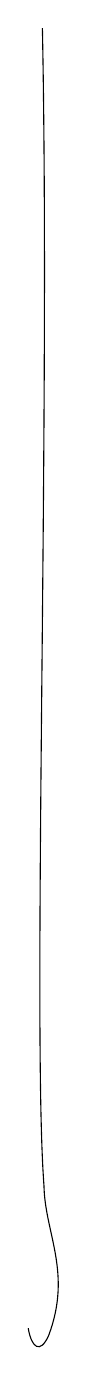
\begin{tikzpicture}[x=1cm,y=1cm]
\draw (0,0) .. controls (0.10,-5.0) and (-0.13,-12.7) .. (0.02,-14.7) .. controls (0.03,-15.3) and (0.38,-15.8) .. (0.08,-16.6) .. controls (-0.03,-16.85) and (-0.14,-16.75) .. (-0.18,-16.51);
\end{tikzpicture}}}
Les classes d'isomorphie de tels \unsure{éléments} \deleted{\unsure{s'identifient}}\inserted{\unsure{correspondent}} biunivoquement aux classes de $M$-conjugaison des scindages de l'extension (287) de $\Gamma$ par $\widetilde{\mathcal M}$. De façon précise, à un $(E,\Theta_{\widetilde{\mathcal M}})$ est associé \unsure{canonique|canoniquement} un \deleted{$\unsure{M}$} homomorphisme de $M$-ensembles
\[
(290)\qquad
\diagram{\begin{tikzcd}[column sep=large]
E \arrow[r] & \operatorname{Scind}(\widetilde{\mathcal M}\ \unsure{\text{ext.}}\ \text{de }\Gamma\ \text{par }M)
\end{tikzcd}}
\]
dont l'image est la classe de conjugaison \unsure{décrivant} la classe d'isomorphie envisagée. \deleted{\unsure{L'image}}\inserted{L'hom} (290) \unsure{se|de} factorise par $M^\Gamma\backslash E$ en un \uline{mono}
\[
(291)\qquad
\diagram{\begin{tikzcd}[column sep=large]
M^\Gamma\backslash E \arrow[r,hook] & \operatorname{Scind}(\widetilde{\mathcal M}\ \text{ext. de }\Gamma\ \text{par }M)
\end{tikzcd}},
\]
et si $M^\Gamma=0$, on voit que $E$ se reconstitue canoniquement à partir de la classe de

\margin{131}

\begin{center}
\small
131\\
\texttt{https://grothendieck.umontpellier.fr}\\
Université de Montpellier, UMR CNRS 5149, Case courrier 051, Place Eugène Bataillon\\
34095 Montpellier cedex 5 - France
\end{center}

\scanpage{133}
\mspage{714}

conjugaison envisagée. L'opération \inserted{(affine)} de $\widetilde{\mathcal M}$ sur $E$ \inserted{(définie par $\Theta_{\widetilde{\mathcal M}}$)} n'est autre que l'opération \deleted{de} \inserted{(\unsure{induite} par la)} conjugaison sur \inserted{l'ens} des scindages (qui bien entendu ne fait pas sortir d'une classe de $M$-conjugaison, $\overline{\mathrm m}$ en conjuguant par des éléments quelconques de $\widetilde{\mathcal M}$).
\margin{\figure{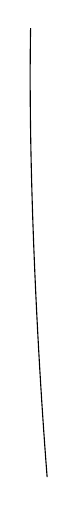
\begin{tikzpicture}[x=1cm,y=1cm]
\draw (0,0) .. controls (-0.03,-1.65) and (0.07,-3.9) .. (0.21,-5.7);
\end{tikzpicture}}}

\uline{Corollaire} Supposons que l'on ait
\[
(292)\qquad \underbrace{H^0(\widetilde\Gamma,M)}_{M^\Gamma}=H^1(\widetilde\Gamma,M)=0
\]
i.e. que \deleted{\unsure{toutes|tous}} deux scindages d'une ext. triviale de $\widetilde\Gamma$ par $M$ soient conjugués par un élément unique de $M$. Cela implique \inserted{donc (à cause de $M^\Gamma=\unsure{\{0\}|0}$)} que la catégorie des $\mathcal X'$, ou encore celle des couples $(E,\Theta_{\widetilde{\mathcal M}})$, est rigide, \deleted{Alors les classes} \inserted{i.e. un objet est connu à isom.} unique près quand on connait sa classe d'isomorphie. Ceci posé, les classes d'isomorphie en question \deleted{correspondent}\inserted{(i.e. les classes} de \deleted{$M$-\unsure{conj|conj.}} conjugaison des scindages de \deleted{biunivoquement} l'ext. $\widetilde{\mathcal M}$ de $\Gamma$ par $M$) correspondent biunivoquement aux groupes quotients $\widetilde{\widetilde{\mathcal M}}$
\margin{\figure{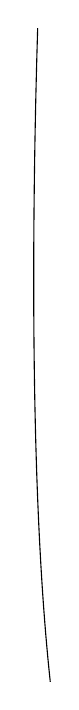
\begin{tikzpicture}[x=1cm,y=1cm]
\draw (0,0) .. controls (-0.06,-1.95) and (-0.12,-5.7) .. (0.16,-8.3);
\end{tikzpicture}}}

\margin{132}

\begin{center}
\small
132\\
\texttt{https://grothendieck.umontpellier.fr}\\
Université de Montpellier, UMR CNRS 5149, Case courrier 051, Place Eugène Bataillon\\
34095 Montpellier cedex 5 - France
\end{center}
